\documentclass[uplatex,a4paper]{jsarticle}
\usepackage[dvipdfmx]{graphicx}
\usepackage{minted}
\usepackage{here}
\usepackage[left=20mm,right=20mm]{geometry}
\title{パターン認識 4月25日の課題}
\author{48176404 井原央翔}
\begin{document}
\definecolor{bg}{gray}{0.95}
\maketitle
\section*{課題1}
Pythonソースコードを以下に示す。
\inputminted[linenos=true,breaklines=true,bgcolor=bg,fontsize=\footnotesize]{python}{assignment1.py}
\subsection{$\Sigma_i=\sigma^2I$の場合}
同一の等方性の正規分布に基づいて2組の2次元ベクトル1000個($X_0$および$X_1$)を生成し、それらの期待値$M_i$および共分散行列$\Sigma_i$を推定した。
識別関数
\[
g_i(X) = -\frac{1}{2} \left( X - M_i \right) \Sigma_i^{-1} \left( X - M_i \right)^T -\frac{1}{2} \log\left( \left| \Sigma_i \right| \right) + \log\left(P\right)
\]
を考え、$g_0 > g_1$が成り立つ領域は$\omega_0$、それ以外の領域は$\omega_1$とした。
これに基づき、$P_0$が$0.1$、$0.3$、$0.5$の各場合について$X_i$の分類を行い、その正誤を含めて散布図を図\ref{fig:ass1_case1}にプロットした。
図\ref{fig:ass1_case1}に、$M_i$および$\Sigma_i$を正規分布のパラメータとして計算される確率密度$N_X$、$g_0-g_1$の等高線プロットを重ねた。
\begin{figure}[H]
\begin{center}
\begin{tabular}{ccc}
\begin{minipage}{0.33\linewidth}
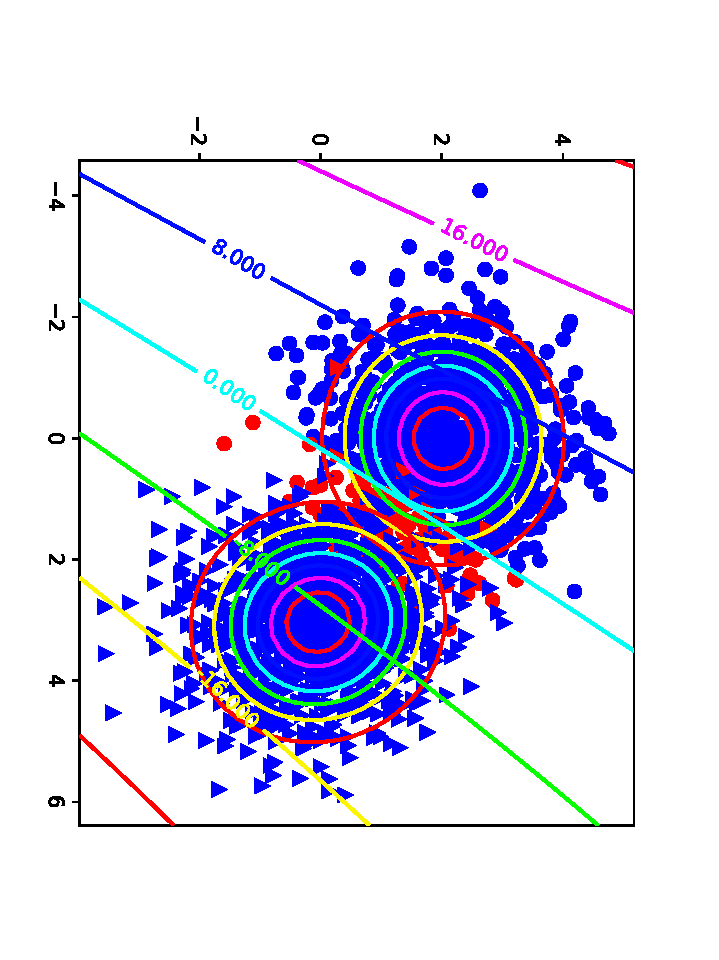
\includegraphics[width=6cm]{Model1_10.pdf}
\end{minipage}
\begin{minipage}{0.33\linewidth}
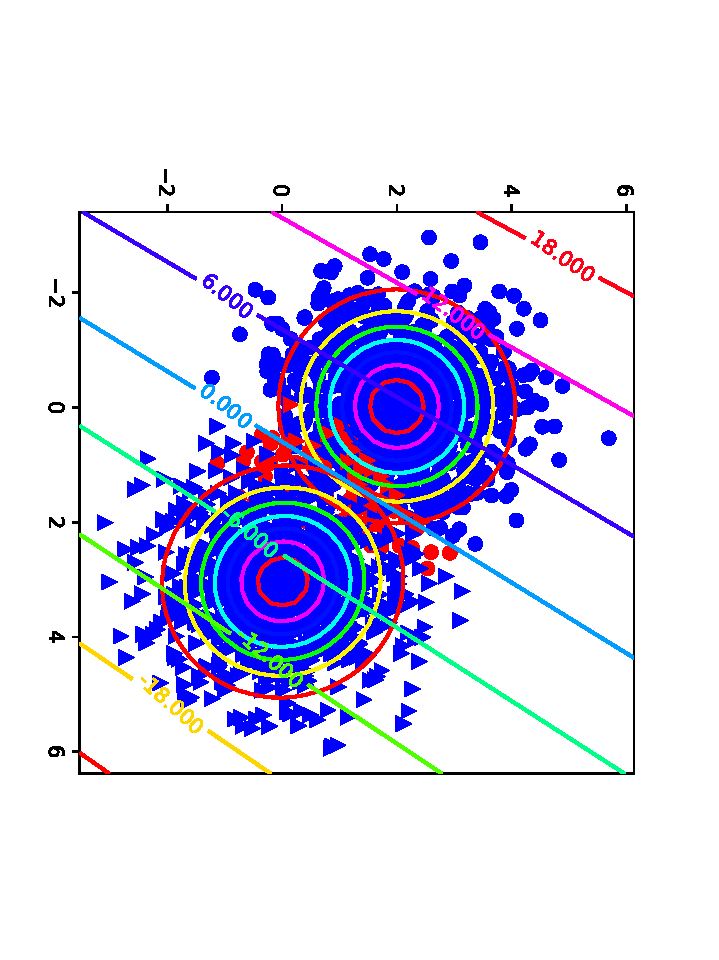
\includegraphics[width=7cm]{Model1_30.pdf}
\end{minipage}
\begin{minipage}{0.33\linewidth}
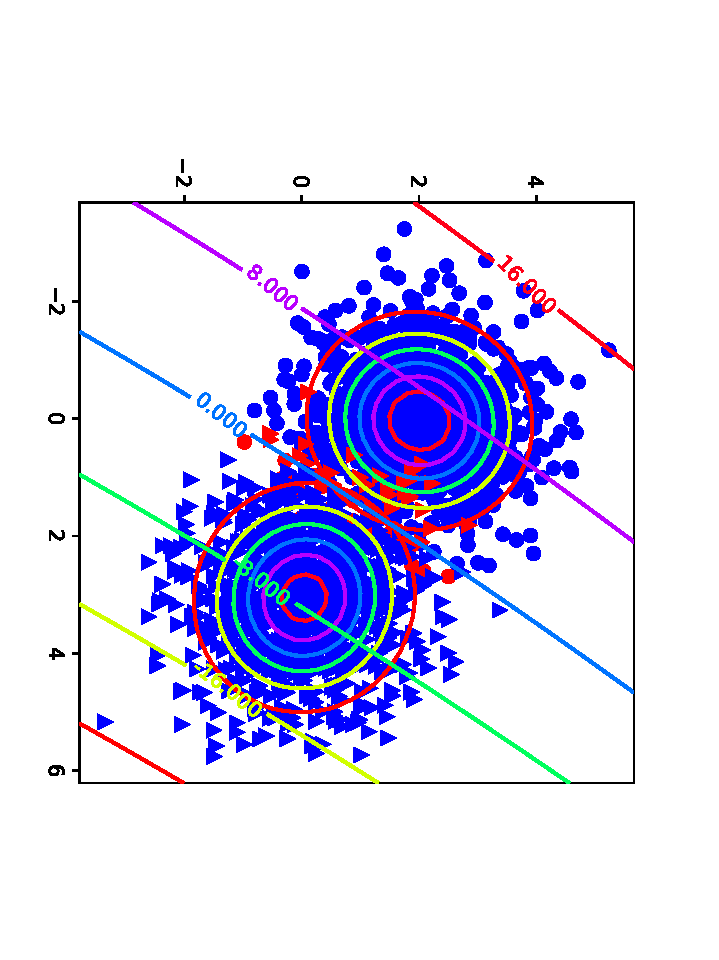
\includegraphics[width=7cm]{Model1_50.pdf}
\end{minipage}
\end{tabular}
\end{center}
\caption{Case1:$\Sigma_i=\sigma^2I$の場合の出力}
\label{fig:ass1_case1}
\end{figure}
\subsection{$\Sigma_i=\Sigma$の場合}
同一の異方性の正規分布に基づいて$X_0$および$X_1$を生成し、$P_0$が$0.1$、$0.3$、$0.5$の各場合について、Case1と同様の手順によって図\ref{fig:ass1_case2}を得た。
\begin{figure}[H]
\begin{center}
\begin{tabular}{ccc}
\begin{minipage}{0.33\hsize}
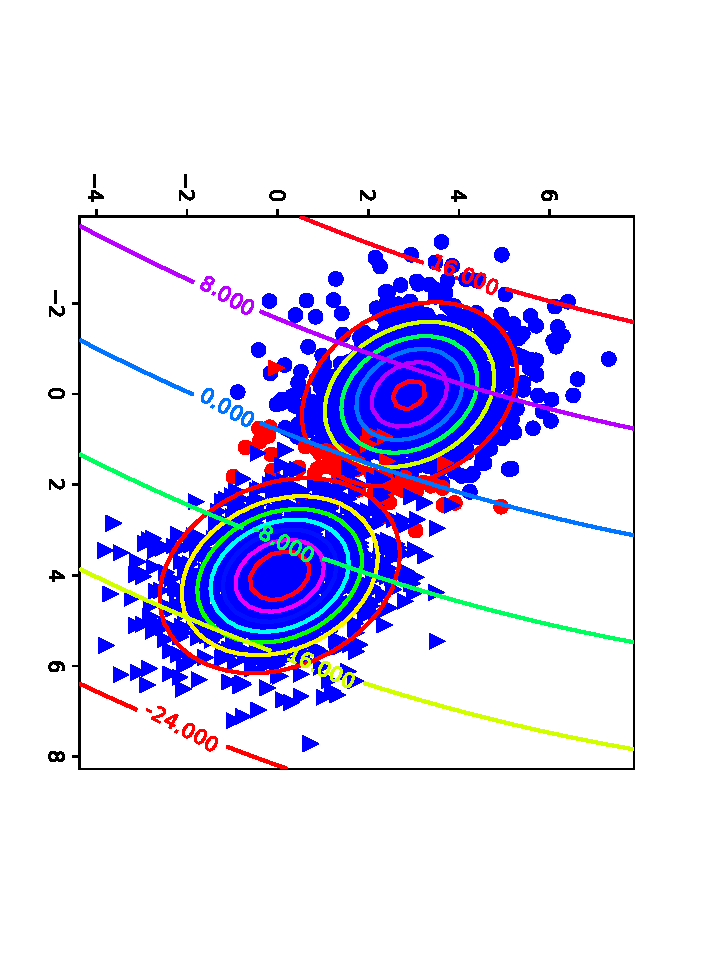
\includegraphics[width=7cm]{Model2_10.pdf}
\end{minipage}
\begin{minipage}{0.33\hsize}
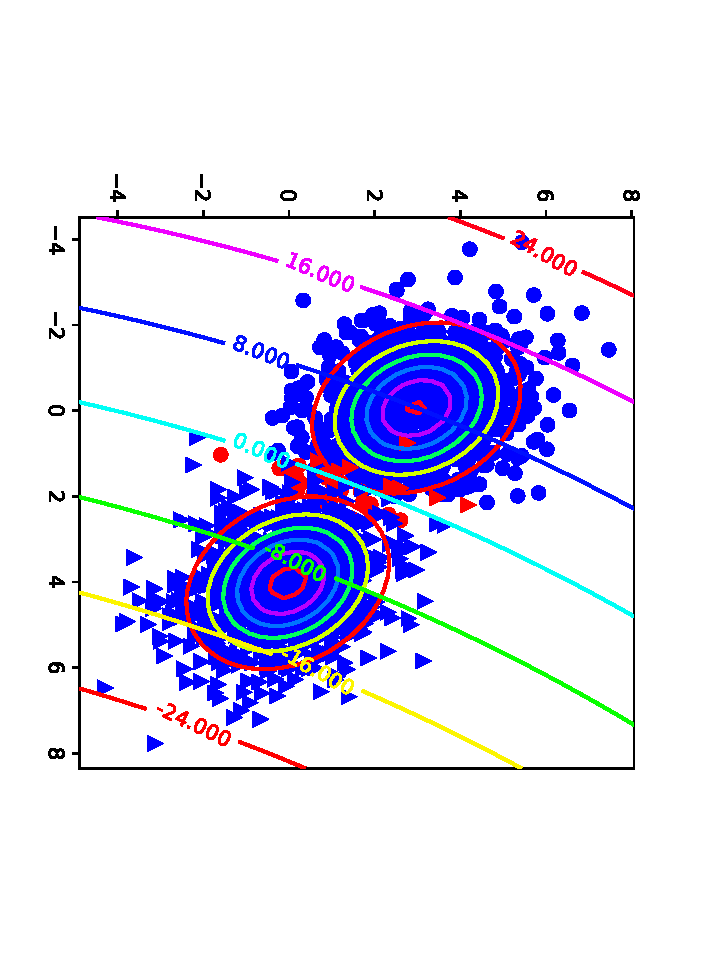
\includegraphics[width=7cm]{Model2_30.pdf}
\end{minipage}
\begin{minipage}{0.33\hsize}
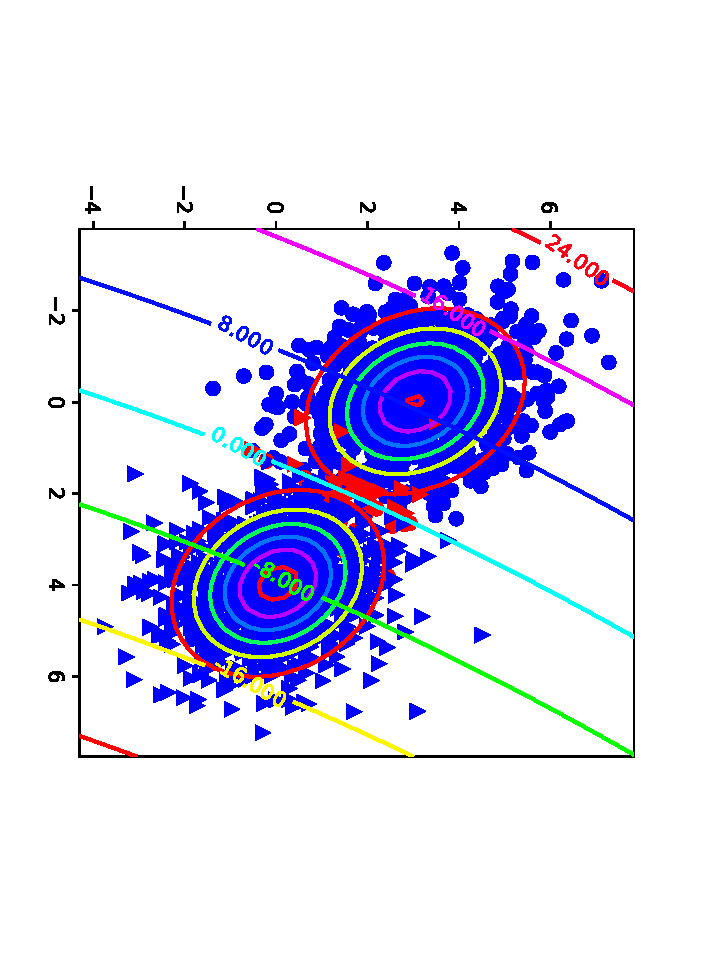
\includegraphics[width=7cm]{Model2_50.pdf}
\end{minipage}
\end{tabular}
\caption{Case2:$\Sigma_i=\Sigma$の場合の出力}
\label{fig:ass1_case2}
\end{center}
\end{figure}
\subsection{任意の$\Sigma_i$の場合}
異なる異方性の正規分布に基づいて$X_0$および$X_1$を生成し、$P_0$が$0.1$、$0.3$、$0.5$、$0.7$、$0.9$の各場合について、Case1と同様の手順によって図\ref{fig:ass1_case3}を得た。
\begin{figure}[H]
\begin{center}
\begin{tabular}{ccc}
\begin{minipage}{0.33\hsize}
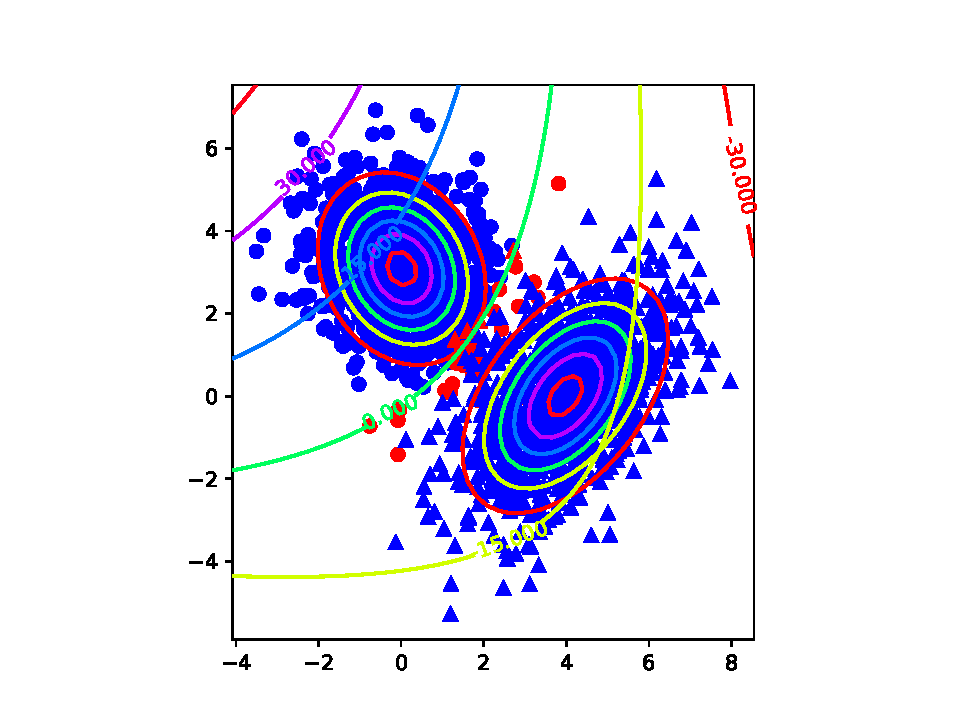
\includegraphics[width=7cm]{Model3_10.pdf}
\end{minipage}
\begin{minipage}{0.33\hsize}
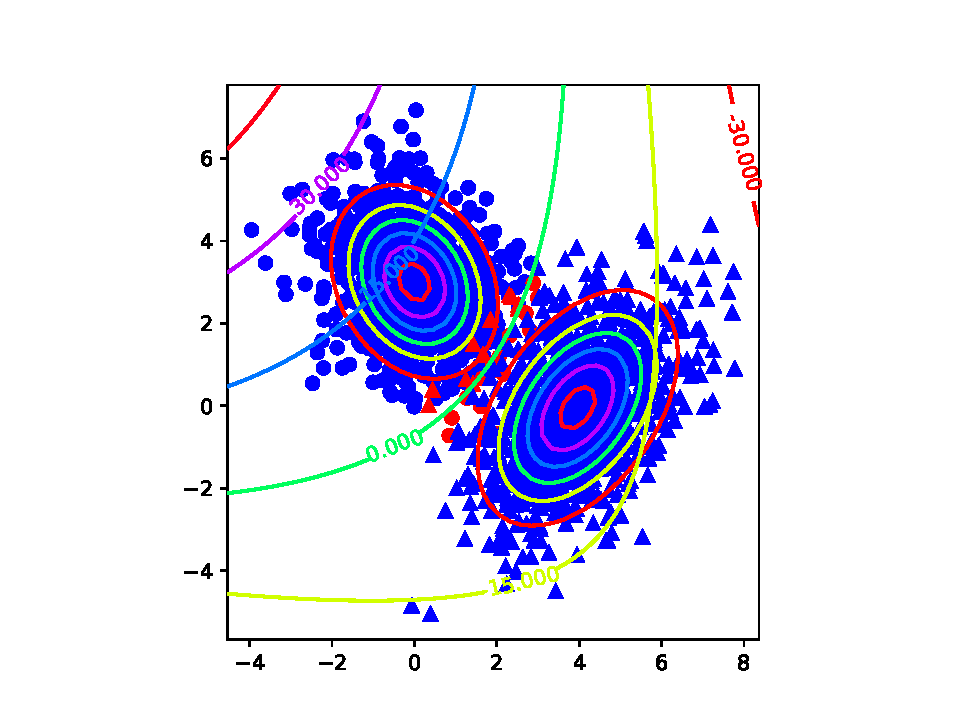
\includegraphics[width=7cm]{Model3_30.pdf}
\end{minipage}
\begin{minipage}{0.33\hsize}
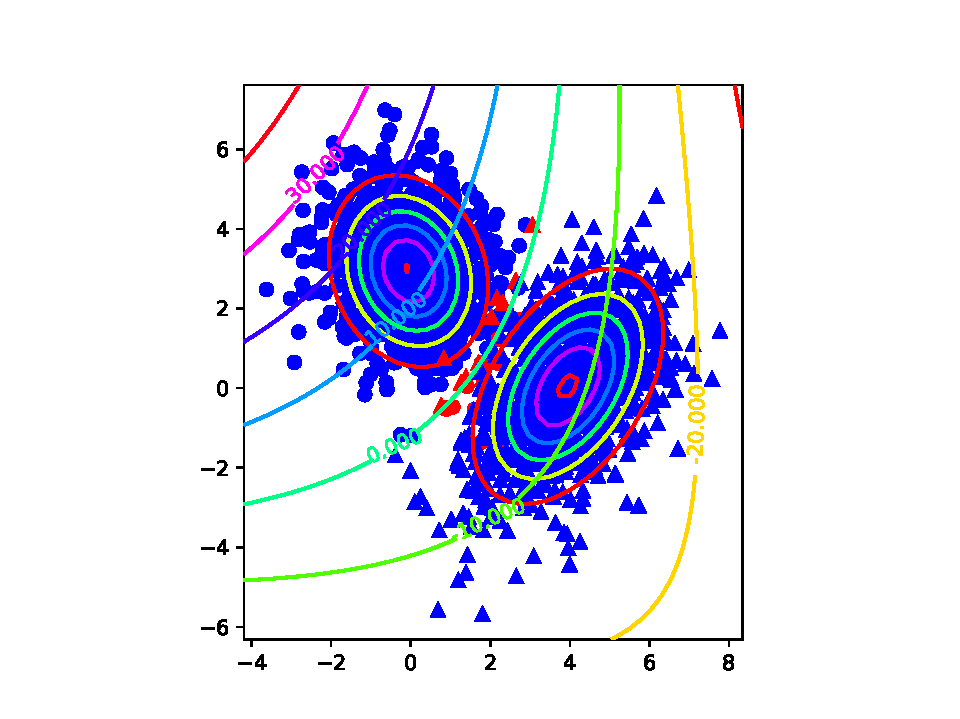
\includegraphics[width=7cm]{Model3_50.pdf}
\end{minipage}
\end{tabular}
\begin{tabular}{cc}
\begin{minipage}{0.33\hsize}
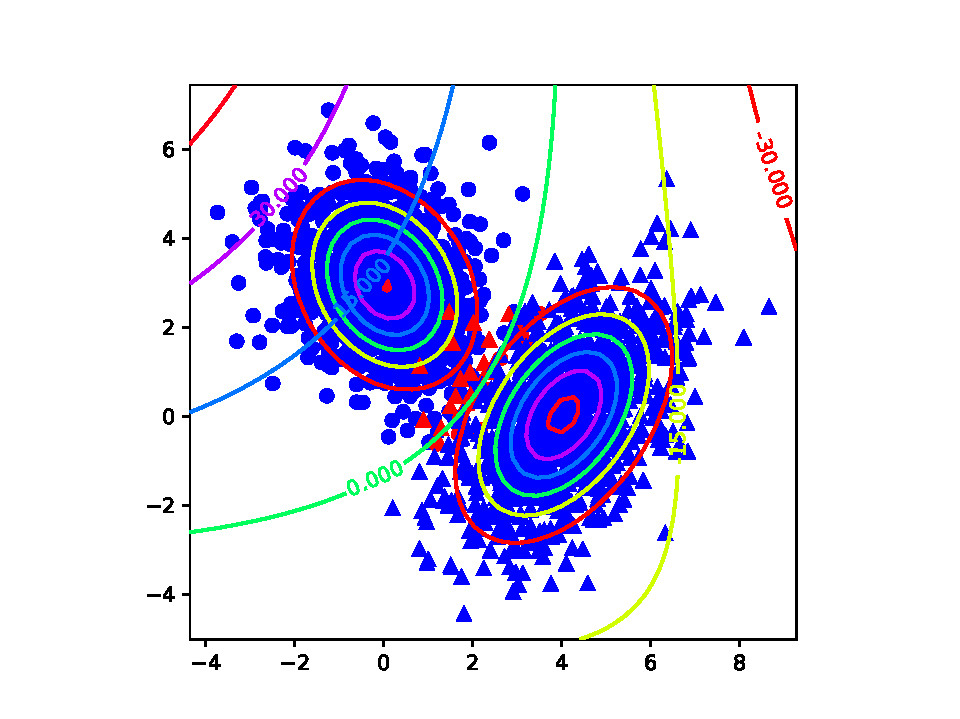
\includegraphics[width=6cm]{Model3_70.pdf}
\end{minipage}
\begin{minipage}{0.33\hsize}
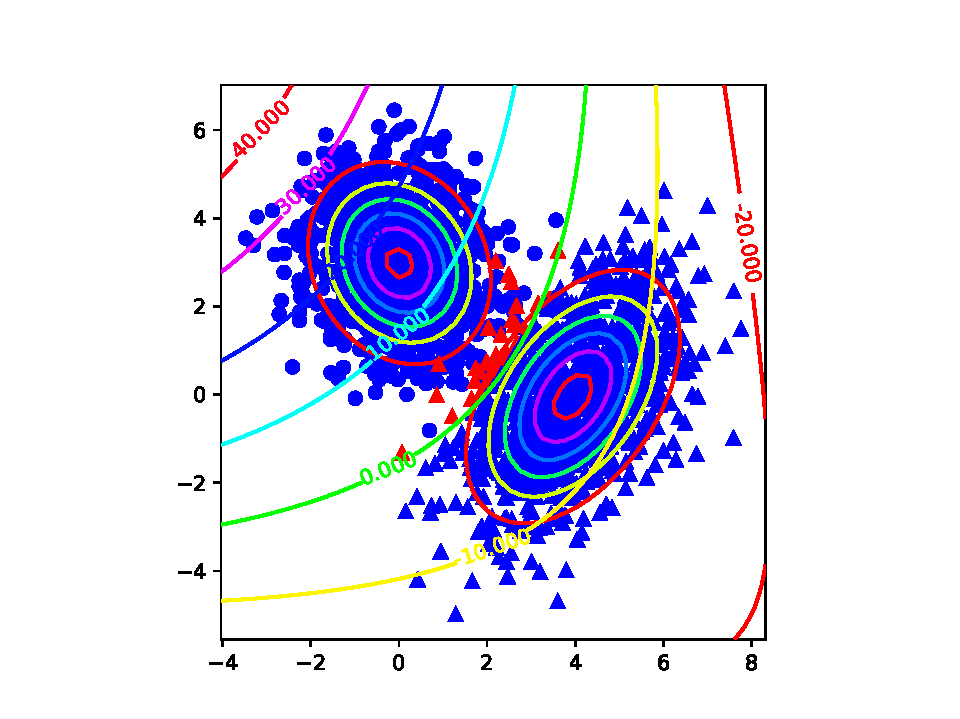
\includegraphics[width=7cm]{Model3_90.pdf}
\end{minipage}
\end{tabular}
\caption{Case3:$\Sigma_i$が任意の場合の出力}
\label{fig:ass1_case3}
\end{center}
\end{figure}
\section*{課題2}
Pythonソースコードを以下に示す。
\inputminted[linenos=true,breaklines=true,bgcolor=bg,fontsize=\footnotesize]{python}{assignment2.py}

\end{document}
